% Straight up stealing preamble from Eli Holmes 
%%%%%%%%%%%%%%%%%%%%%%%%%%%%%%%%%%%%%%START PREAMBLE THAT IS THE SAME FOR ALL EXAMPLES
\documentclass{article}

%Required: You must have these
\usepackage{Sweave}
\usepackage{graphicx}
\usepackage{tabularx}
\usepackage{hyperref}
\usepackage{natbib}
\usepackage{pdflscape}
\usepackage{array}
\usepackage{gensymb}
%\usepackage[backend=bibtex]{biblatex}
%Strongly recommended
 %put your figures in one place
 
%you'll want these for pretty captioning
\usepackage[small]{caption}

\setkeys{Gin}{width=0.8\textwidth} %make the figs 50 perc textwidth
\setlength{\captionmargin}{30pt}
\setlength{\abovecaptionskip}{0pt}
\setlength{\belowcaptionskip}{10pt}
% manual for caption http://www.dd.chalmers.se/latex/Docs/PDF/caption.pdf

%Optional: I like to muck with my margins and spacing in ways that LaTeX frowns on
%Here's how to do that
 \topmargin -2cm     
 \oddsidemargin -0.04cm   
 \evensidemargin -0.04cm  % same as oddsidemargin but for left-hand pages
 \textwidth 16.59cm
 \textheight 22.94cm 
 %\pagestyle{empty}       % Uncomment if don't want page numbers
 \parskip 7.2pt           % sets spacing between paragraphs
 %\renewcommand{\baselinestretch}{1.5} 	% Uncomment for 1.5 spacing between lines
\parindent 0pt% sets leading space for paragraphs
\usepackage{setspace}
%\doublespacing

%Optional: I like fancy headers
\usepackage{fancyhdr}
\pagestyle{fancy}
\fancyhead[LO]{Phenological sequences}
\fancyhead[RO]{2017}

%%%%%%%%%%%%%%%%%%%%%%%%%%%%%%%%%%%%%%END PREAMBLE THAT IS THE SAME FOR ALL EXAMPLES

%Start of the document
\begin{document}

% \SweaveOpts{concordance=TRUE}
\bibliographystyle{/Users/aileneettinger/citations/Bibtex/styles/amnat.bst}
\title{Supplemental materials for \\ Phenological sequences: How early-season events define those that follow} 
\author{A.K. Ettinger, S. Gee, and E.M. Wolkovich}
%\date{\today}
\maketitle  %put the fancy title on
%\tableofcontents      %add a table of contents
%\clearpage
%%%%%%%%%%%%%%%%%%%%%%%%%%%%%%%%%%%%%%%%%%%%%%%%%%%
\renewcommand{\thetable}{S\arabic{table}}
\renewcommand{\thefigure}{S\arabic{figure}}


%\section*{Supplemental Methods}

%\section* {Supplemental Results}


%\section{Bibliography}
%\bibliography{/Users/aileneettinger/citations/Bibtex/mylibrary}

\section* {Supplemental Tables}
%EMW: Also, the giving of all the equations is a little hard; consider including some of the min/max ones and give the equations in a supplemental table?
% latex table generated in R 3.2.4 by xtable 1.8-2 package
% Wed Sep  6 21:43:09 2017
\begin{table}[ht]
\centering
\caption{Summary of linear models for relationships between later phenophases and earlier phenophases, as shown in Figure 3 in the main text. Linear models were fit with the species-level mean day-of-year of the later phenological stages as the response variable,
and mean day-of-year of earlier phenostage as the explanatory variable.} 
\label{table:prevphase}
\begin{tabular}{|p{0.35\textwidth}|p{0.1\textwidth}|p{0.07\textwidth}|p{0.07\textwidth}|p{0.07\textwidth}|}
  \hline
previous phenostage model & intercept & slope & r\textsuperscript{2} & p \\ 
  \hline
leafout vs. budburst & 65.84 & 15.33 & 0.44 & <0.001 \\ 
  flowering vs. budburst & 3.18 & 65.27 & 0.17 & 0.039 \\ 
  fruiting vs. budburst & -80.31 & 96.27 & 0.23 & 0.016 \\ 
  senescence vs. budburst & 243.88 & 45.52 & 0.03 & 0.427 \\ 
  flowering vs. leafout & -105.28 & 80.04 & 0.30 & 0.005 \\ 
  fruiting vs. leafout & -107.19 & 134.07 & 0.16 & 0.051 \\ 
  senescence vs. leafout & 237.39 & 60.89 & 0.02 & 0.484 \\ 
  fruiting vs. flowering & 5.21 & 31.73 & 0.54 & <0.001 \\ 
  senescence vs. flowering & 261.65 & 19.36 & 0.04 & 0.332 \\ 
  senesence vs. fruiting & 253.54 & 14.00 & 0.14 & 0.06 \\ 
   \hline
\end{tabular}
\end{table}% latex table generated in R 3.2.4 by xtable 1.8-2 package
% Wed Sep  6 21:43:09 2017
\begin{table}[ht]
\centering
\caption{Summary of linear models for relationships between later phenophases and inter-phenophase duration, as shown in Figure 4 in the main text. Linear models were fit with the species-level mean day-of-year of the later phenological stages as the response variable, and the number of days in each previous inter-phenophase duration as the explanatory variable.} 
\label{table:interphase}
\begin{tabular}{|p{0.35\textwidth}|p{0.1\textwidth}|p{0.07\textwidth}|p{0.07\textwidth}|p{0.07\textwidth}|}
  \hline
inter-phenophase model & intercept & slope & r\textsuperscript{2} & p \\ 
  \hline
leafout vs. leafout-budburst & 128.977 & 2.330 & 0.035 & 0.374 \\ 
  flowering vs. leafout-budburst & 144.522 & 8.307 & 0.001 & 0.874 \\ 
  fruiting vs. leafout-budburst & 276.477 & 15.903 & 0.047 & 0.3 \\ 
  senescence vs. leafout-budburst & 281.980 & 5.338 & 0.004 & 0.763 \\ 
  flowering vs. flowering-leafout & 129.280 & 1.591 & 0.926 & <0.001 \\ 
  fruiting vs. flowering-leafout & 245.864 & 9.920 & 0.250 & 0.011 \\ 
  senescence vs. flowering-leafout & 278.627 & 3.698 & 0.034 & 0.381 \\ 
  fruiting vs. fruiting-flowering & 143.556 & 15.426 & 0.740 & <0.001 \\ 
  senescence vs. fruiting-flowering & 258.294 & 8.647 & 0.242 & 0.013 \\ 
  senesence vs. senescence-fruiting & 282.109 & 3.231 & 0.047 & 0.296 \\ 
   \hline
\end{tabular}
\end{table}\clearpage

\section* {Supplemental Figures}

\begin{figure}[h]
  \centering
  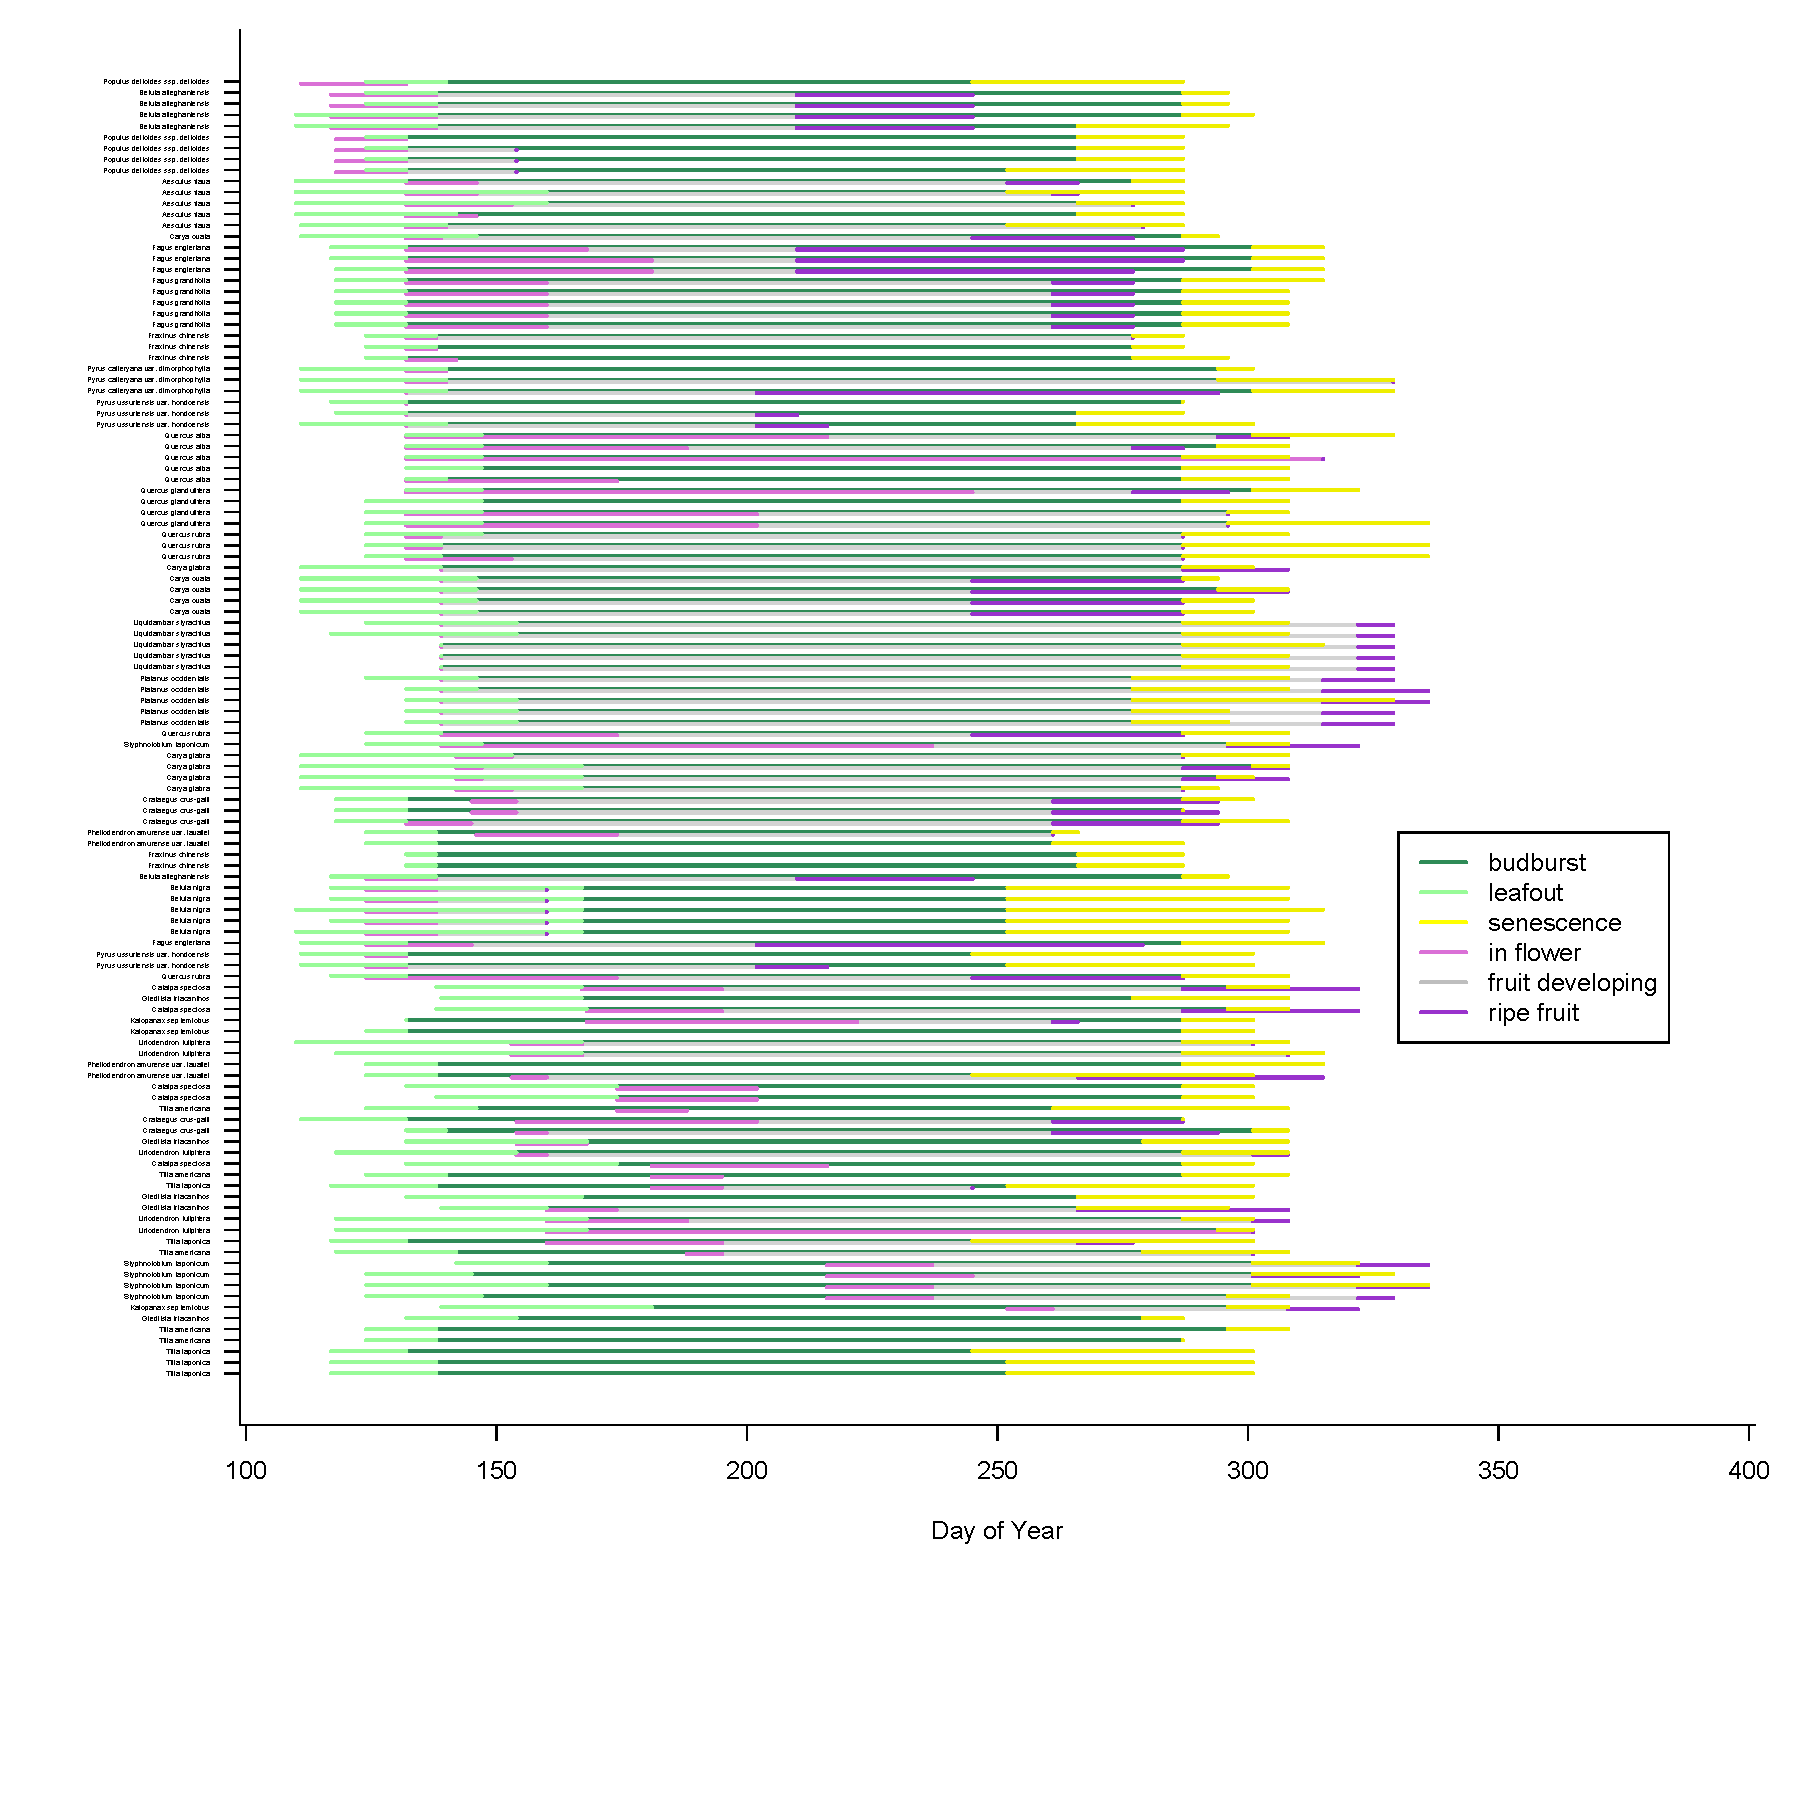
\includegraphics{../analyses/figures/grosea_repsort_ripefruit_ind_legend.pdf}
  \caption{\textbf{Individual tree phenology during the 2015 growing season, ordered by species-level mean first-flower dates.} Growth phenology is shown for budburst (from its mean start day-of-year to the mean start day-of-year for leafout, across all individuals within a species), leafout (from the mean day-of-year when fully-expanded leaves were first observed through the start of senescence), and senescence (from the mean day-of-year when leaves first began changing color through the mean day-of-year when more than 95 percent of leaves on the tree had changed color). Reproductive phenology is shown for flowering (from the mean day-of-year when flowers first appeared to the mean day-of-year when fruits first appeared, across all individuals within a species) and fruiting (from the mean day-of-year when fruits first appeared to the mean day-of-year when more than 95 percent of fruits were first observed as ripe).}
 \label{fig:focind}
\end{figure}
  
%%%%%%%%%%%%%%%%%%%%%%%%%%%%%%%%%%%%%%%%
\end{document}
%%%%%%%%%%%%%%%%%%%%%%%%%%%%%%%%%%%%%%%%
